%% GS-NDN --- IEEE conference manuscript.
%%
%% Every number here was read from results/*.json after the final 20-seed
%% campaign, not copied from README.md or RESULTS.md. Both of those lagged the
%% data at least once during development, which is why the rule exists.
%%
%% Figures live in paper/figures/; refresh them with
%%     python experiments/make_figures.py --sync-paper
%% Setup, metrics and catalog construction replicate Amadeo et al. (IEEE IoT
%% Magazine, Mar 2026); see the comparison-basis subsection for what is
%% deliberately stricter and why absolute numbers are not compared.
\documentclass[conference]{IEEEtran}
\IEEEoverridecommandlockouts

\usepackage{cite}
\usepackage{amsmath,amssymb}
\usepackage{graphicx}
\usepackage{booktabs}
\usepackage{url}
\usepackage[hidelinks]{hyperref}
\usepackage{balance}
\usepackage[T1]{fontenc}
\usepackage{mathptmx}

%% Default \medmuskip carries plus/minus, so justification squeezes the space
%% around \pm on a tight line and opens it on a loose one -- "11.1+-7.5" and
%% "24.9 +- 7.3" in the same paragraph. Fixed widths make every one match.
\thinmuskip=3mu
\medmuskip=4mu
\thickmuskip=5mu

%% NDN names are typeset with \path, from url (loaded by hyperref). It breaks
%% after every slash, so a long name cannot become one unbreakable box wider
%% than a column -- which is what stretched the spaces around it. A hand-rolled
%% macro was tried here first and got the terminator wrong, emitting a trailing
%% slash and no breakpoints at all.
\urlstyle{tt}
\newcommand{\ndn}[1]{\path{#1}}

%% Figures live in paper/figures/, copied from results/figures/ by
%% experiments/make_figures.py --sync-paper. The paper directory is therefore
%% self-contained: uploading it alone to Overleaf compiles.
\graphicspath{{figures/}}

%% \linebreakand is not a built-in IEEEtran command; it must be defined once,
%% here in the preamble, before \begin{document}. It closes the current
	%% author-alignment environment and reopens a new one, which is what forces
	%% a row break between authors in the \author block below.
	\makeatletter
	\newcommand{\linebreakand}{%
	\end{@IEEEauthorhalign}
	\hfill\mbox{}\par
	\mbox{}\hfill\begin{@IEEEauthorhalign}
	}
	\makeatother
	
	\begin{document}
		
		\title{Gossip-Scaled Semantic Forwarding in\\Named Data Networking}
		
		%% ---------------------------------------------------------------------------
		%% CAMERA-READY author block. Replace the two "Given Name Surname" and
		%% "email address or ORCID" placeholders below with real values before
		%% submission. Layout is 3 authors in the first row, 2 in the second, via
		%% \linebreakand (defined in the preamble above).
		%% ---------------------------------------------------------------------------
		\author{
			\IEEEauthorblockN{1st Given Name Surname}
			\IEEEauthorblockA{
				\small\textit{Dept. Electrical and Computer Engineering}\\
				\small\textit{University of Tehran}\\
				\small\textit{Tehran, Iran}\\
				\small\textit{email address or ORCID}
			}
			\and
			\IEEEauthorblockN{2nd Given Name Surname}
			\IEEEauthorblockA{
				\small\textit{Dept. Electrical and Computer Engineering}\\
				\small\textit{University of Tehran}\\
				\small\textit{Tehran, Iran}\\
				\small\textit{email address or ORCID}
			}
			\and
			\IEEEauthorblockN{Mohammad R. Shakournia}
			\IEEEauthorblockA{
				\small\textit{Dept. Electrical and Computer Engineering}\\
				\small\textit{University of Tehran}\\
				\small\textit{Tehran, Iran}\\
				\small\textit{shakournia@ut.ac.ir}
			}
			\linebreakand
			\IEEEauthorblockN{Pooya Jamshidi}
			\IEEEauthorblockA{
				\small\textit{Dept. Electrical and Computer Engineering}\\
				\small\textit{University of Tehran}\\
				\small\textit{Tehran, Iran}\\
				\small\textit{pooya.jamshidi@ut.ac.ir}
			}
			\and
			\IEEEauthorblockN{Shahpour Rahmani}
			\IEEEauthorblockA{
				\small\textit{Dept. Electrical and Computer Engineering}\\
				\small\textit{University of Tehran}\\
				\small\textit{Tehran, Iran}\\
				\small\textit{shahpour.rahmani@ut.ac.ir}
			}
		}
		
		\maketitle
		
		\begin{abstract}
			Named Data Networking drops a request whose name does not match a
			router's forwarding table. Two hospitals naming the same sensor
			differently cannot reach each other's data. Matching names by embedding
			similarity fixes this, but it puts a sentence encoder in the forwarding
			path on every miss. A per-router cache does not solve the cost. Split the
			same traffic across more routers, and each cache sees less of it. Over a
			short run, the network calls the encoder more often as it grows, not
			less.
			
			We share each resolved mapping over gossip instead, once, and only after
			a returned Data packet confirms it. Over a 60\,s run at 16 edge routers,
			this holds encoder-call growth to $+9.9\%$, against $+59.6\%$ for a
			per-router cache, cutting inferences by $27.7\%$. The saving has limits:
			it falls to $6.5\%$ over 600\,s, and it reverses below about four edge
			routers.
			
			The same verification step yields two more results. First, the feedback
			a router learns from is biased, not just noisy. A producer's refusal
			cannot tell ``this name is not mine'' apart from ``this name is mine,
			but not in that wording''---a distinction NDN's Network Nack was never
			built to carry. Second, a gossiped mapping can be checked, so a router
			can audit its peers from verdicts it already has. This cuts a persistent
			poisoning attacker's damage by $1.2\times$ to $2.0\times$, more as the
			attack grows. It is an attenuation, not a hard bound: we tested the
			rate-independence a bound predicts, and it failed.
		\end{abstract}
		
		\begin{IEEEkeywords}
			Named Data Networking, semantic forwarding, anti-entropy gossip, conformal
			prediction, Byzantine resilience.
		\end{IEEEkeywords}
		
		\section{Introduction}
		
		Named Data Networking (NDN)~\cite{jacobson2009ccn,zhang2014ndn} forwards on
		names. A name that does not match the Forwarding Information Base (FIB) gets
		dropped. A client asking for \ndn{/hospital/temp-sensor/room-101} gets nothing
		from a network that advertises
		\ndn{/smart-hospital/floor-1/temperature/room-101}, though the data is one hop
		away. Amadeo \emph{et al.}~\cite{amadeo2026} fix this by embedding names and
		matching them with cosine similarity, caching each resolution in an
		\emph{Embedding Store} at the router that made it.
		
		That design has a scaling problem their own conclusion leaves as future work.
		A per-router cache only learns from the traffic that router sees. Add more
		edge routers without adding traffic, and every cache sees a thinner slice, so
		it learns less. The network ends up calling the encoder more often overall.
		We measured this: $+59.6\%$ more inferences from 1 to 16 edge routers on one
		catalog, $+67.4\%$ on the other, for the same offered load.
		
		Our premise is simple: the fix is a shared cache, not a bigger one. NDN
		already gives us what makes sharing safe. A semantic match is only a hypothesis; a returned Data packet provides
		producer-side confirmation that the selected service responded. Gossiping only producer-confirmed mappings
		prevents unsupported semantic guesses from becoming shared state. That is also what lets the similarity threshold stay
		permissive without the usual cost.
		
		However, existing NDN synchronization mechanisms do not answer the question
		that semantic forwarding introduces: when is a learned name-to-route mapping
		safe to share? Synchronizing an incorrect semantic resolution can amplify a
		local recognition error into a network-wide routing error. Conversely, waiting
		for perfect semantic certainty defeats the purpose of approximate matching.
		The key design question is therefore not how to disseminate state, but how to
		admit semantic state into the shared namespace. We show that producer-confirmed
		responses provide a practical admission signal: they allow routers to exchange
		useful semantic resolutions while retaining an observable failure signal when
		those resolutions are later challenged.
		
		\textbf{Contributions.} We make three claims, each scoped to what we
		measured.
		
		\begin{itemize}
			\item \emph{Sharing substantially limits recognition-cost growth as the network expands} (\S\ref{sec:scaling}). We also
			measure what bounds this: the advantage shrinks with run length and
			reverses below about four edge routers.
			\item \emph{The free labels a forwarding plane calibrates on are biased,
				not just noisy} (\S\ref{sec:bias}), and the bias traces to a specific
			gap in the protocol rather than to noise. We found this defect in our
			own producer model, fixed it, and report where the fix helps and where
			it does not.
			\item \emph{A verifying forwarding plane can audit its own peers}
			(\S\ref{sec:threat}). Byzantine-robust gossip normally cannot catch a
			liar, only bound the damage. A gossiped mapping, unlike a gradient, can
			be checked against what its producer actually says.
		\end{itemize}
		
		\textbf{What we do not claim.} Edge tagging---marking an Interest with its
		resolved prefix so later hops skip the encoder---is Amadeo \emph{et al.}'s
		mechanism; we inherit it. Anti-entropy synchronisation is a decade old in
		NDN~\cite{zhu2013chronosync,hoque2013nlsr}; our gossip layer just carries a
		different payload over it. Learning per-item boundaries under an error
		budget is what vCache~\cite{schroeder2025vcache} does for LLM prompt caching.
		We tried an error budget in place of the similarity threshold. It lost to a
		threshold tuned on one catalog and carried to another, and we report that as
		a withdrawn claim (\S\ref{sec:risk}).
		
		\textbf{Organisation.} Section~\ref{sec:related} places this work against
		semantic forwarding in ICN, the synchronisation layers NDN already has, and
		prior work on learned boundaries and Byzantine-robust gossip.
		Section~\ref{sec:method} describes the simulator, the producer model, and how
		costs were measured. Sections~\ref{sec:scaling}, \ref{sec:bias}
		and~\ref{sec:threat} present the three contributions, each ending with a
		supporting result of its own. Section~\ref{sec:risk} covers the claim we
		withdrew, and Section~\ref{sec:limits} the limitations and where they lead
		next.
		
		\section{Background and Related Work}
		\label{sec:related}
		
		\textbf{Semantic forwarding in ICN.} Fuzzy Interest
		Forwarding~\cite{chan2017fuzzy} matches name components with Word2Vec. It is
		the original statement of this problem. Amadeo \emph{et
			al.}~\cite{amadeo2026} use a sentence encoder instead, settle on a threshold
		of $0.7$, and evaluate a single access router. INF-NDN~\cite{raza2024infndn}
		takes a different path: it routes topic tags through central supernodes,
		concentrating semantic resolution rather than sharing it. Raza \emph{et
			al.}~\cite{raza2025smartnets} pair NLP-based semantic name matching with a
		learned feedforward network, but for FIB distribution and retrieval. Their
		target is prefix compactness and lookup time, not the multi-router encoder
		cost this paper measures. Amadeo \emph{et al.}~\cite{amadeo2026dtn} also
		extend semantic ICN matching to service provisioning across cooperating
		digital twins. That is a different coordination problem from sharing one
		resolution once it has been proven.
		
		\textbf{A note on ``SAF''.} In NDN, SAF already denotes Stochastic Adaptive
		Forwarding~\cite{posch2017saf}. We write ``semantic forwarding'' or name the
		authors instead. Our result files still use the key \texttt{saf}, for
		continuity with earlier work.
		
		\textbf{Synchronisation NDN already has.} Our anti-entropy and
		rumour-spreading pair is the classical epidemic construction of Demers
		\emph{et al.}~\cite{demers1987epidemic}. Its $O(\log N)$ propagation under
		random peer choice~\cite{karp2000rumor} is what Section~\ref{sec:frontier}
		preserves, by keeping one uniform pick. ChronoSync~\cite{zhu2013chronosync}
		and its successors reconcile datasets by exchanging condensed digests.
		NLSR~\cite{hoque2013nlsr} already floods name-prefix reachability over such a
		layer. Moll \emph{et al.}~\cite{moll2022sok} survey how these designs differ.
		Our contribution is not the mechanism; it is the payload and the
		precondition. We share a wording-to-route mapping only after a Data packet
		provides producer-side confirmation. Section~\ref{sec:scaling} measures an unbounded version of
		this sync layer, because ``why not just announce the prefix'' is the first
		objection this design invites.
		
		\textbf{Learned boundaries under an error bound.}
		vCache~\cite{schroeder2025vcache} learns per-item thresholds under a
		user-set error bound, for prompt caching. Finamore \emph{et
			al.}~\cite{finamore2022approximatekey} do error-controlled similarity
		caching in a networking setting. These boundaries are conformal in the
		sense of Vovk \emph{et al.}~\cite{vovk2005alrw}. Pooling calibration across
		parties is federated conformal prediction~\cite{lu2023federated}. The
		drifting variant we evaluate follows adaptive conformal
		inference~\cite{gibbs2021aci}. A threshold tuned on one catalog need not
		hold on another; this is the covariate-shift problem Tibshirani \emph{et
			al.}~\cite{tibshirani2019covariate} treat formally. What is specific to
		NDN is that the labels come free. An LLM cache needs a judge model to check
		whether a hit was correct, which is the cost one was trying to avoid. A
		forwarding plane gets this signal for nothing: whether the producer answers
		or refuses.
		
		\textbf{Biased feedback.} Section~\ref{sec:bias} is an instance of
		missing-not-at-random feedback, the pattern Saito \emph{et
			al.}~\cite{saito2020unbiased} study in implicit-feedback recommendation. A
		route's label depends on a producer's declared vocabulary, and that same
		vocabulary decides whether the request could have been served at all. Our
		contribution is finding this in a forwarding plane and naming the protocol
		gap that causes it.
		
		\textbf{Byzantine-robust gossip.} Robust aggregation, clipping, trimming, a
		bounded per-peer contribution, bounds an adversary's influence without ever
		identifying it. In gossip learning, a neighbour ships a gradient no honest
		node can check. Section~\ref{sec:threat} exploits a difference: a gossiped
		mapping, unlike a gradient, can be checked against what its producer
		actually says.
		
		\section{System Model and Method}
		\label{sec:method}
		
		\subsection{Simulator}
		
		We embed names with MiniLM~\cite{wang2020minilm}, a distilled Sentence-BERT
		model. It is the same model the baseline uses. Each router has a
		single-server FIFO queue. So a strategy that adds work to the forwarding
		path pays for it in queueing delay, not in some fixed constant. A strategy
		is consulted at exactly one point, the FIB miss, and told the outcome
		afterwards. Content Store, PIT, and exact FIB lookup stay identical across
		strategies. So any difference in results is a difference in policy, nothing
		else. The simulator itself is written in Python, as a discrete-event
		kernel with no external network simulator dependency.
		
		Similarity can choose a route. It can never decide that two names mean the
		same object. A semantic hit in the Content Store would hand a client data it
		did not ask for. A semantic hit in the PIT would send data down the wrong
		chain.
		
		\subsection{Costs are measured, not assumed}
		
		Every latency constant here is measured on the machine running the study,
		and tagged as measured or assumed. One MiniLM-L6 inference costs
		$7.045$\,ms. A cosine search over the 50-entry FIB costs $0.0045$\,ms. That
		is a ratio of about $1566$:$1$. So \emph{the encoder is the only cost that
			matters}: any scheme that speeds up the similarity search is optimising a
		rounding error. Our mechanism targets how often the encoder runs, not how
		fast it runs.
		
		\subsection{Producers are modelled, not oracular}
		
		Letting a producer consult ground truth would be the weakest assumption we
		could make. So instead, each producer holds a \emph{declared schema}: the
		instance it serves and the terms it answers to, much like a service
		registry or an OpenAPI description would give. These declarations are
		deliberately incomplete. At coverage $0.7$, a producer leaves $29\%$ of its
		own possible wordings undeclared, and refuses requests that were genuinely
		meant for it. The feedback channel is informative, not correct. That is
		also true of any real deployment, since no producer outside our simulator
		has access to ground truth either.
		
		\subsection{Workload and metrics}
		
		Requests arrive as a Poisson process over a Zipf ($\alpha=1.2$) popularity
		distribution. Each consumer population draws from an overlapping but
		distinct slice of the catalog. Without that overlap, sharing would be
		either trivially redundant or trivially useless. Each catalog holds 50
		services, 300 rewordings, and 350 distractors that no service can satisfy,
		so precision stays measurable.
		
		Scoring is correctness-aware. Every Interest ends in exactly one of four
		states: correct, misdelivered, rejected, or timeout, judged against ground
		truth the routers never see. Distractors are supposed to be rejected, so a
		single accuracy number would reward a strategy that answers nothing. We
		report precision, recall, and false-positive rate separately instead. We
		also report an Interest Satisfaction Rate (ISR): the share of resolvable
		Interests answered correctly, the recall figure above under a different
		name, used because it is the metric the baseline itself reports.
		
		\subsection{Comparison basis}
		\label{sec:basis}
		
		We reproduce the baseline's evaluation setting rather than invent our own:
		the access-edge topology, one-way latencies (10\,ms client-to-router,
		20\,ms router-to-provider), the 50-entry FIB, the 30--300 Interests/s
		range, the Zipf skew of $1.2$, a disabled Content Store, and an unbounded
		PIT all come from Amadeo \emph{et al.}~\cite{amadeo2026}. Our catalogs
		match their construction exactly: 50 services, one canonical name and six
		rewordings each, 350 satisfiable names, and an equal number of unrelated
		ones.
		
		We report their metrics, mapped onto ours. Their \emph{service discovery
			time} is our Interest-satisfaction time; it decomposes the same way. Their
		\emph{processing time} is our encoder-invocation count times the measured
		inference cost, plus queueing. Their \emph{share of Interests forwarded on
			the first attempt} is our satisfaction rate, with one deliberate
		difference: they count an Interest successful once it is forwarded and
		answered, while we also require the Data to come from the correct service.
		A confident match to the wrong room's sensor counts as success under their
		definition and as a misdelivery under ours. Only our definition can be
		tuned against that failure at all.
		
		\textbf{Absolute numbers are not comparable across the two papers, so we do
			not compare them.} They report near-complete forwarding at
		$\mathrm{Th}=0.7$; ours yields recall of $0.866$ and $0.804$ at that
		threshold. The gap is in the rewordings, not the method. Theirs are
		synonym substitutions. Ours also drop hierarchy levels, reorder
		components, and abbreviate, and a seventh family draws on published IoT
		vocabularies. Every comparison here stays inside one harness, never
		against a number from another paper.
		
		\subsection{Cross-validation}
		
		A hand-written simulator can be internally consistent and still model NDN
		incorrectly. So we cross-check the transport layer, which is not our
		contribution, against ndnSIM, on the same topology, delays, and request
		pattern, with semantic resolution turned off. Median round-trip times
		agree to within $0.11$\,ms once we account for the $1$\,ms producer
		service time our model charges.
		
		All results come from 20 seeded runs with 95\% confidence intervals, and
		they reproduce across processes. During development we found three
		defects where interpreter-salted iteration order leaked into the event
		queue. A regression test now compares metrics from two child processes run
		under different \texttt{PYTHONHASHSEED} values, to catch any recurrence.
		
		\section{Scaling: Sharing versus Caching}
		\label{sec:scaling}
		
		\begin{figure}[t]
			\centering
			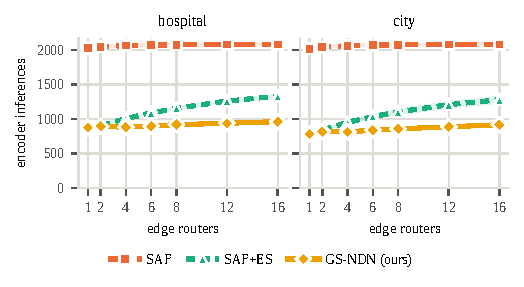
\includegraphics[width=\columnwidth]{fig_scaling.pdf}
			\caption{Encoder invocations against edge routers. The per-router cache grows
				with the network; gossiped sharing stays nearly flat.}
			\label{fig:scaling}
		\end{figure}
		
		Fig.~\ref{fig:scaling} shows the effect this paper is built around. Semantic
		forwarding without a cache pays for every FIB miss, so it has nothing to erode
		and grows $+2.8\%$ and $+3.1\%$ from 1 to 16 edge routers. The per-router cache
		thins as routers multiply and grows $+59.6\%$ on hospital and $+67.4\%$ on
		city. Sharing holds that to $+9.9\%$ and $+17.3\%$, removing $27.7\%$ and
		$28.3\%$ of all inferences at 16 edge routers. The claim is independent of any
		threshold or error budget: it is a property of how many times the encoder
		runs.
		
		\subsection{Two conditions that bound it}
		
		\textbf{The horizon.} A cold cache costs one inference per router per wording:
		$N$ routers pay it $N$ times, but they pay it once. Over 600\,s instead of
		60\,s the per-router cache grows $+14.4\%$ rather than $+55.2\%$, and gossip's
		saving at 16 edge routers falls from $25.6\%$ to $6.5\%$ (city: $26.8\%$ to
		$9.2\%$). The ordering never reverses, but the magnitude does: sharing pays a
		network that is large and still learning its catalog.
		
		\textbf{Network size.} At a single edge router there is nobody to share with,
		and anti-entropy costs $4$--$5\%$ more inferences than a plain per-router
		cache. The benefit appears from about four edge routers upward.
		
		\subsection{Is the decay an artifact of a closed catalog?}
		
		A natural hypothesis is that the decay is an artifact of a finite catalog: once
		every router has met all 300 rewordings there is nothing left to learn. We
		tested it by introducing wordings over the run instead of making them all
		askable at $t=0$, drawn from an independent random stream so only \emph{which}
		wording a request uses changes. The hypothesis is false, and instructively so:
		a slower arrival rate lowers the saving at \emph{every} horizon instead of
		sustaining it, from $25.6\%$ (closed) to $3.0\%$ (one new wording every 5\,s)
		at 60\,s, monotone across the grid and on both catalogs. Gossip's saving comes
		from the \emph{backlog} of resolutions some routers hold and others do not, and
		a closed catalog at $t=0$ is the largest backlog obtainable.
		
		\subsection{Would a more aggressive sync layer do better?}
		
		NDN already ships anti-entropy synchronisation, so the obvious objection is to
		turn it on and drop this layer. We bound that with an arm in which every router
		reconciles with every peer each round with no cap per exchange. It removes
		\emph{fewer} inferences than the bounded protocol ($21.0\%$ against $25.6\%$ at
		16 edge routers) while sending $1.2$--$1.6\times$ the bytes. Anti-entropy at
		fanout 2 already reaches everyone in $O(\log N)$ rounds, and what limits the
		saving is how many distinct wordings the network has yet to see---a quantity no
		amount of synchronisation changes. What does the work here is \emph{what} is
		shared and \emph{when}, a mapping shared only once a Data packet proved it, not
		how aggressively it is shared.
		
		\subsection{A Pareto frontier, not an operating point}
		\label{sec:frontier}
		
		The gossip period is a degree of freedom, and a single value would hide a trade
		worth seeing. Sweeping it from $0.25$ to $5$\,s at 16 edge routers moves the
		saving from $24.4\%$ to $18.0\%$ while gossip traffic falls from $933$ to
		$433$\,kB. At 4 edge routers the saving is flat across the same range
		($8.5$--$9.6\%$), and a longer period is nearly free there. The exchange rate
		between bytes and inferences therefore depends on network size, and a
		conclusion drawn at one operating point would have been wrong at the other.
		The chosen $0.5$\,s is also Pareto-optimal among the points measured: $0.25$\,s
		is worse on \emph{both} axes.
		
		\textbf{Delta-biased peer selection.} Once converged, the modal anti-entropy
		exchange is two agreeing digests and no payload. Ranking partners by how far
		behind they are redirects those exchanges and costs no messages, since the
		sender already keeps the watermark. One pick of \texttt{fanout} stays uniform:
		a purely greedy rule is no longer an epidemic process and can starve a peer
		that never tops the ranking. This is the only mechanism we tested that moves
		the frontier outward instead of along it. Paired at 16 edge routers it saves
		$11.1 \pm 7.5$ inferences while sending $3.68 \pm 0.96\%$ fewer bytes at
		$0.5$\,s, and $24.9 \pm 7.3$ inferences at $1.0$\,s (20/20 seeds), with
		satisfaction unchanged. The magnitude is honestly small---$1$--$1.5\%$ of
		invocations and $3\%$ of bytes, not a headline result---and it helps only in
		the mid-range network sizes where the ranking has something to bite on, which
		is the pattern this explanation predicts.
		
		\subsection{Latency and energy}
		\label{sec:scaling-latency}
		
		Encoding on every FIB miss saturates the forwarding path: p95 round-trip time
		rises from $79$ to $172$\,ms between 30 and 300 Interests/s, while cached and
		gossiped variants stay flat at $78$--$83$\,ms. The knee sits just past 200
		Interests/s, independently reproducing the bottleneck the baseline reports
		beyond roughly 210 for the same encoder---agreement we did not tune for, and
		evidence the cost model is calibrated. On the radio model of Askar \emph{et
			al.}~\cite{askar2024sef}, with encoder energy charged at measured CPU draw,
		GS-NDN uses $634$\,J against $735$\,J uncached and $654$\,J for a per-router
		cache, at higher satisfaction. A character $n$-gram control reaches $0.791$
		satisfaction where MiniLM reaches $0.969$: it resolves abbreviations and fails
		on true synonymy, which is what the encoder pays for.
		
		\section{Calibrating from Free Labels}
		\label{sec:risk}
		
		A threshold is a property of the catalog it was tuned on. $0.7$ works on the
		baseline's catalog, but on ours it yields recall of only $0.866$ and
		$0.804$. A single number also has to serve every route at once, and routes
		are not alike. Some services sit alone in embedding space, so a loose score
		is safe. Others have near-identical siblings, so a high score is really a
		coin flip. Every semantic forwarding decision is an experiment the network
		answers on its own, so $(\text{score},\text{verdict})$ pairs accumulate for
		free. An operator can then set an error budget $\varepsilon$ instead of a
		fixed threshold. For route $r$, we take the lowest score whose upper
		confidence bound on the error rate, among observations at or above it,
		still stays within $\varepsilon$. We use a Wilson bound rather than the
		normal approximation, since the normal approximation gives a route with no
		observed errors a bound of exactly zero after only a dozen observations. We
		also shrink each route toward a pooled boundary, at a rate set by its own
		evidence.
		
		Two results follow from this. Only one of them is good.
		
		\textbf{Risk control deadlocks without exploration.} A boundary set too
		high blocks exactly the decisions that would produce the evidence needed to
		lower it. Left unexplored, the controller settles into refusing everything
		and stays there, reaching only $0.732$ satisfaction at $\varepsilon=0.02$.
		Tightening $\varepsilon$ further changes nothing, since it is already
		refusing everything it can. Spending just $5\%$ of refused decisions on
		exploration reaches $0.818$ instead. This is not an estimator bug; it is
		simply what happens when a system learns only from its own past choices. We
		report these exploratory forwards separately, since they are decisions the
		budget itself did not cover.
		
		\textbf{The efficiency claim was tested and withdrawn.} The budget holds
		out-of-sample in all fourteen tests we ran: two catalogs, crossed with
		seven error budgets $\varepsilon \in \{0.02, 0.05, 0.10, 0.15, 0.20, 0.30,
		0.40\}$. But against a threshold tuned on one catalog and carried over to
		the other, the controller Pareto-dominates in \emph{none} of those fourteen
		comparisons, while the transferred threshold dominates in seven of them.
		What survives is narrower than we hoped: the controller needs no labelled
		sample from the domain it runs on. An operator who already has one should
		just tune a threshold instead.
		
		\section{The Feedback is Biased, Not Just Noisy}
		\label{sec:bias}
		
		This is the finding the paper stands on, alongside the scaling result. It
		came from a defect we found in our own producer model.
		
		A producer refusing a semantically-resolved Interest can have two distinct
		reasons, and a plain refusal signal cannot tell them apart. ``This name is
		not mine'' is a routing fact: the mapping that sent the Interest here was
		simply wrong. ``This name is mine, but not in that wording'' is not a
		routing fact at all: the route was correct, and only the phrasing fell
		outside what the producer had declared. Collapsing these two makes every
		gap in a producer's vocabulary look like evidence against a route that
		was, in fact, right. HTTP separates 404 from 406 for exactly this reason,
		and DNS separates NXDOMAIN from NODATA. NDN's Network Nack was never built
		to carry this kind of distinction: its standard reason codes cover
		forwarding-plane conditions, like congestion or a missing route, not a
		producer's own semantic judgment. Semantic forwarding is what first makes
		that judgment necessary.
		
		\textbf{The distinction has to be one a producer can actually make.} Our
		first implementation tested whether the producer published \emph{the
			prefix the router had chosen}. But a misroute satisfies that test by
		construction, since that prefix is exactly why the Interest was routed
		there in the first place. At full declaration coverage, where a genuine
		wording gap is nearly impossible, we measured 132 of 157 refusals
		reporting ``unknown wording'' about a route that was simply wrong. Only 2
		were the case that label actually exists for, and the routing-error label
		never fired once. The channel was carrying almost no information at all.
		
		What a producer genuinely knows is which \emph{instance} it is attached
		to: the room, the junction, the meter. A request that does not name that
		instance is not meant for this service, no matter how it is worded. That
		test turns out to be exact in our runs: every instance mismatch we found
		was either a real misroute or an unsatisfiable distractor, with no false
		positives at all. This one change turns a dead channel into an
		informative one. At coverage $0.5$, $291$ refusals are now correctly
		labelled as routing errors, and $546$ as wording gaps, $71\%$ of which are
		genuine.
		
		\textbf{The residue inverts.} A producer serving temperature readings in
		room 101, asked for humidity in that same room, cannot tell a metric it
		truly does not serve apart from a synonym of its own it simply forgot to
		declare. The base rate of genuine gaps among such refusals moves from
		$0.021$ at full coverage up to $0.711$ at half coverage, and the right
		policy for handling them inverts along with it. Ignoring ambiguous
		refusals gains $0.07$ satisfaction at coverage $0.5$ ($0.844$ against
		$0.774$), but it \emph{costs} $0.014$ at full coverage on city ($0.963$
		against $0.978$). Declaration coverage is a property of other
		organisations' service registries, something an operator simply cannot
		observe.
		
		We tried to close this gap with inverse propensity weighting, estimating
		a propensity per route. The attempt failed, but in an informative way:
		the estimated weight sat between $0.414$ and $0.470$ across \emph{every}
		regime we tested, on both catalogs. A correct route at low coverage both
		serves often and gets refused often, so a route-conditioned ratio barely
		moves at all. What actually does move is a single, network-wide base
		rate. We report this regime inversion as an open problem, one whose
		magnitude we have measured but not one we have a mechanism to fix.
		
		\subsection{Schema drift}
		\label{sec:bias-drift}
		
		Producer relocation hurts every strategy equally, since FIB withdrawal
		invalidates a stale mapping before any producer even gets the chance to
		refuse it. Schema drift is different: a producer quietly narrows what it
		answers to, with no routing event at all. This removes that confound, and
		there, verification's advantage finally shows up: $+0.0042 \pm 0.0018$
		satisfaction on hospital (16 of 20 seeds) and $+0.0124 \pm 0.0045$ on city
		(19 of 20), paired seed by seed. Nothing in the routing plane can observe
		a schema drift on its own; feedback is the only signal that can.
		
		\section{Threat Model and Peer Reputation}
		\label{sec:threat}
		
		\begin{figure}[t]
			\centering
			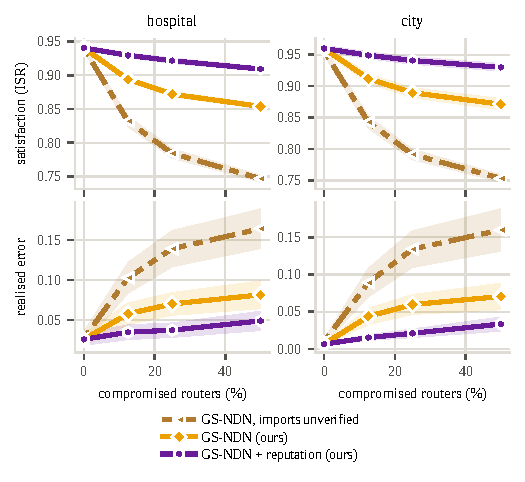
\includegraphics[width=\columnwidth]{fig_robust.pdf}
			\caption{Satisfaction and realised error under a persistent poisoning attacker.
				Reputation is free at zero compromise and recovers most of the attack's cost
				thereafter.}
			\label{fig:robust}
		\end{figure}
		
		\subsection{Threat model}
		
		\textbf{What the attacker controls.} A fixed share of routers, chosen
		uniformly at random. Each is a full participant, holding real keys and real
		peer relationships, so nothing here is defeated just by authenticating the
		channel. Each one behaves correctly on the forwarding path and lies only
		into gossip. A router that drops traffic outright is a different problem, a
		denial-of-service problem the ICN literature already
		treats~\cite{ghali2014poisoning}, and including it here would confound the
		measurement.
		
		\textbf{What it can do.} It injects fabricated mappings and fabricated
		calibration evidence, and re-injects both every round, so a single
		retraction settles nothing. It also knows the catalog well enough to target
		names clients actually request. That is the strong assumption in this
		model.
		
		\textbf{What it cannot do.} It cannot forge another router's identity,
		partition the network, observe traffic it does not carry, or make a
		producer answer a name it does not actually publish. This boundary matters
		for \S\ref{sec:bias}: the refusal signal is authored by the producer
		itself, at the application layer, so a compromised \emph{router} cannot
		forge one. What a compromised \emph{producer} could do, on the other hand,
		is left unmeasured.
		
		\textbf{What limits damage structurally.} A router's own confirmed mappings
		always outrank anything it is merely told by a peer. This is not a defence
		we added specifically against this attack; it simply falls out of
		gossiping only what a returned Data packet has already confirmed.
		
		\subsection{Verification-grounded reputation}
		
		Byzantine-robust gossip normally has to defend without any ground truth,
		bounding an adversary's influence without ever actually identifying it. A
		gossiped mapping is different: it is falsifiable, and the producer answers
		it directly. We charge each refusal to the peer that supplied the mapping,
		and we never reinstall a pair the router has disproved first-hand. Trust is
		a Wilson \emph{lower} bound on a peer's success rate, mirroring the upper
		bound on error from \S\ref{sec:risk}: both bound in whichever direction
		costs us more. A peer with no history yet is believed by default, and this
		is deliberate: distrusting every unaudited peer would break the bootstrap
		that gossip depends on in the first place.
		
		Calibration evidence needs a different defence, since a single observation
		about a route is not immediately falsifiable on its own. So no single peer
		may supply more than a quarter of a route's calibration window. This bounds
		its contribution by construction, not by detection.
		
		\begin{table}[t]
			\caption{Satisfaction and realised error against compromised share, 8 edge
				routers. ``Imports unverified'' is the behaviour before we extended
				verification to mappings learned over gossip.}
			\label{tab:robust}
			\centering
			\small
			\begin{tabular}{@{}lrrrr@{}}
				\toprule
				compromised & $0\%$ & $12.5\%$ & $25\%$ & $50\%$ \\
				\midrule
				\multicolumn{5}{@{}l}{\emph{hospital}, satisfaction} \\
				Imports unverified & $0.940$ & $0.832$ & $0.784$ & $0.747$ \\
				GS-NDN & $0.941$ & $0.894$ & $0.872$ & $0.854$ \\
				\quad$+$ reputation & $0.941$ & $\mathbf{0.930}$ & $\mathbf{0.922}$ & $\mathbf{0.909}$ \\
				\multicolumn{5}{@{}l}{\emph{hospital}, realised error} \\
				Imports unverified & $0.027$ & $0.103$ & $0.139$ & $0.164$ \\
				GS-NDN & $0.026$ & $0.058$ & $0.070$ & $0.081$ \\
				\quad$+$ reputation & $0.026$ & $\mathbf{0.035}$ & $\mathbf{0.037}$ & $\mathbf{0.049}$ \\
				\midrule
				\multicolumn{5}{@{}l}{\emph{city}, satisfaction} \\
				Imports unverified & $0.956$ & $0.843$ & $0.791$ & $0.753$ \\
				GS-NDN & $0.960$ & $0.912$ & $0.890$ & $0.871$ \\
				\quad$+$ reputation & $0.960$ & $\mathbf{0.949}$ & $\mathbf{0.941}$ & $\mathbf{0.930}$ \\
				\multicolumn{5}{@{}l}{\emph{city}, realised error} \\
				Imports unverified & $0.010$ & $0.089$ & $0.134$ & $0.160$ \\
				GS-NDN & $0.007$ & $0.044$ & $0.060$ & $0.071$ \\
				\quad$+$ reputation & $0.007$ & $\mathbf{0.015}$ & $\mathbf{0.021}$ & $\mathbf{0.033}$ \\
				\bottomrule
			\end{tabular}
		\end{table}
		
		Table~\ref{tab:robust} and Fig.~\ref{fig:robust} show the effect. At $50\%$
		compromise, reputation recovers $0.162$ of the $0.194$ satisfaction the
		attack costs on hospital ($84\%$), and $0.177$ of $0.207$ on city ($86\%$),
		measured at the single injection rate used throughout this table and
		figure; \S\ref{sec:threat-attenuation} sweeps that rate and shows the
		recovered share is not a fixed constant, so these two figures describe one
		operating point, not a general guarantee. It also cuts realised error by
		$40\%$ and $52\%$. Crucially, it costs nothing when nobody is attacking:
		$0.941$ against $0.941$. That single number is what decides whether the
		mechanism can safely be left switched on all the time. It also works for
		the reason we expect: the count of distrusted peers rises linearly with
		the compromised share, reaching $29.3$ at $50\%$.
		
		\subsection{An attenuation, not a breakdown bound}
		\label{sec:threat-attenuation}
		
		It is tempting to formalise this residual as a hard bound. Each pair of an
		honest router and a compromised neighbour admits at most $k$ mappings
		before the liar is finally cut off, where $k$ is the trust prior. That
		gives admitted poison $\lesssim 2Ef(1-f)k$, for $E$ adjacencies and
		compromised fraction $f$: quadratic in $f$, and, in principle,
		\emph{independent of the injection rate}.
		
		We tested both halves of that claim. The mechanism half holds up: sweeping
		$k$ over $\{1,2,4,8,16\}$ moves surviving poison monotonically from $494$
		to $1067$, so the admission fee really is the knob that matters.
		\textbf{Rate invariance, however, fails.} Taking the attacker from 1 to 16
		fabricated mappings per round raises the defended arm's realised error by
		$1.43\times$ on hospital and $1.91\times$ on city. A true bound, counted
		purely in pairs, should not move with rate at all; ours clearly does. So we
		do not claim a breakdown point here.
		
		What does survive is an attenuation whose value \emph{grows} with attack
		intensity. The undefended arm rises $2.35\times$ and $3.25\times$ over that
		same range, so the ratio between defended and undefended widens: from
		$1.24\times$ at the lowest rate to $2.04\times$ at the highest on hospital,
		and from $1.72\times$ to $2.93\times$ on city. In other words, the defence
		is worth more the harder it is attacked.
		
		The sweep also points to a better prior than intuition alone would suggest.
		A fee of $k=1$ is best under active attack, but on a clean network it
		falsely distrusts $10.9$ honest peers and degrades sharing by $3\%$. $k=2$
		distrusts only $1.1$ peers, for a cost of just $0.06\%$, while still
		realising $0.037$ error against $k=4$'s $0.044$. We use $k=2$. This choice
		only becomes visible once we look at the honest-network control; the
		attack column alone would have argued for $k=1$ instead.
		
		%% Balance the two columns of the final page so the bibliography ends level.
		%% This has to be issued from the FIRST column of that page: balance.sty warns
		%% and silently does nothing when it is reached in the second, which is what
		%% happened while it sat at the end of the conclusion.
		\balance
		
		\section{Limitations and Future Work}
		\label{sec:limits}
		
		\textbf{Our synonyms are easier than standardised ones.} Our catalogs use
		a lexicon we wrote ourselves. To test whether it flatters the encoder, we
		added rewordings from Brick, SAREF, Project Haystack, and W3C SSN/SOSA.
		They are markedly harder: on city, rank-1 recognition drops to $0.578$ for
		ontology-derived wordings, against $0.920$ for our own. This confirms the
		concern rather than removing it; every recognition number here should be
		read as an upper bound.
		
		\textbf{Provenance is not implemented.} Our threat model names one other
		defence: signing an observation so a lie traces back to its origin, not to
		whichever honest peer last relayed it. We do not have that. A router that
		penalises the peer a bad mapping arrived from cannot yet tell an
		originator from an honest relay, so the reputation mechanism in
		\S\ref{sec:threat} defends against a source, not the wider network that
		source can hide behind. A deployment facing this threat model needs
		provenance; we only show that the attack lands, and by how much. A
		signed, per-hop provenance field on each gossiped mapping is the direct
		next step.
		
		\textbf{A compromised producer is unmeasured.} Producers are trusted
		about their own services throughout. A producer that lies about its own
		schema sits outside the threat model of \S\ref{sec:threat}, which
		controls only routers. Covering that case would need a separate admission
		check on the producer side.
		
		\textbf{The encoder guard is a trade, not a win.} Refusing to pool
		calibration scores across routers with different encoders yields lower
		satisfaction \emph{and} lower realised error than pooling them naively
		($0.948$/$0.023$ against $0.951$/$0.027$, at a quarter heterogeneous). For
		an error-budget system that trade is defensible, but it is not a clean
		improvement.
		
		\section{Conclusion}
		\label{sec:conclusion}
		
		Sharing producer-confirmed resolutions through gossip, rather than caching
		them independently at each router, substantially limits recognition-cost
		growth as the network expands under the evaluated conditions. We identify the
		two factors that bound this benefit: network size and learning horizon. The
		same producer feedback signal that enables controlled sharing also provides a
		source of calibration evidence and peer-audit information for the forwarding
		plane. However, this feedback is not simply noisy; it is biased because
		existing refusal signalling does not distinguish routing errors from
		unexpressed producer vocabulary. We show that correcting this bias can help
		only under regimes determined by declaration coverage, a quantity that may be
		unavailable to operators. Finally, we report two mechanisms that did not
		improve their intended objective under our evaluation, highlighting that
		understanding failure modes is as important as demonstrating successful
		designs.
		
		\bibliographystyle{IEEEtran}
		\bibliography{references}
		
	\end{document}